% Taller de magnitudes: desarrollo a mano del estudiante + complementos de lo que faltaba.
% Compilar desde esta carpeta:  tectonic entrega_con_complementos.tex
\documentclass[11pt,a4paper]{article}

\usepackage[spanish,es-nodecimaldot,es-tabla]{babel}
\usepackage{fontspec}
\usepackage{amsmath}
\usepackage{siunitx}
\usepackage{booktabs}
\usepackage{graphicx}
\usepackage{float}
\usepackage[font=small,labelfont=bf]{caption}
\usepackage[margin=2.2cm]{geometry}
\usepackage{microtype}
\usepackage[most]{tcolorbox}
\usepackage[hidelinks]{hyperref}

\sisetup{output-decimal-marker={.}, group-separator={\,}, group-minimum-digits=4}
\graphicspath{{fotos/}{../resultados/}}

% Boxes: what the student did, and what is added.
\newtcolorbox{revision}[1][]{colback=green!4!white, colframe=green!45!black, fonttitle=\bfseries,
  title={Revisión de lo hecho}, #1}
\newtcolorbox{complemento}[1][]{colback=blue!4!white, colframe=blue!55!black, fonttitle=\bfseries,
  title={Complemento: lo que faltaba}, #1}

\newcommand{\autor}{Nombre del estudiante}

\title{Astronomía para Todos\\[4pt]\large Taller de ejercicios sobre magnitudes\\
\normalsize Desarrollo a mano y complementos}
\author{\autor}
\date{3 de noviembre de 2026}

\begin{document}
\maketitle

\noindent Este documento reúne el desarrollo hecho a mano (fotos de las hojas) y, después de cada
punto, lo que faltaba para completarlo:
\begin{itemize}
  \item los recuadros \textcolor{green!45!black}{\textbf{verdes}} revisan lo hecho;
  \item los recuadros \textcolor{blue!55!black}{\textbf{azules}} agregan lo que faltaba.
\end{itemize}
Los puntos 1 a 3 estaban resueltos y solo necesitan agregados menores. El punto 4 no estaba en las
hojas y se agrega completo. En el punto 5 la hoja de trabajo estaba llena; faltaban las marcas en la
foto y la conclusión sobre la edad.

\tableofcontents

% =====================================================================
\section{Puntos 1 a 3: desarrollo a mano}

\begin{figure}[H]
\centering
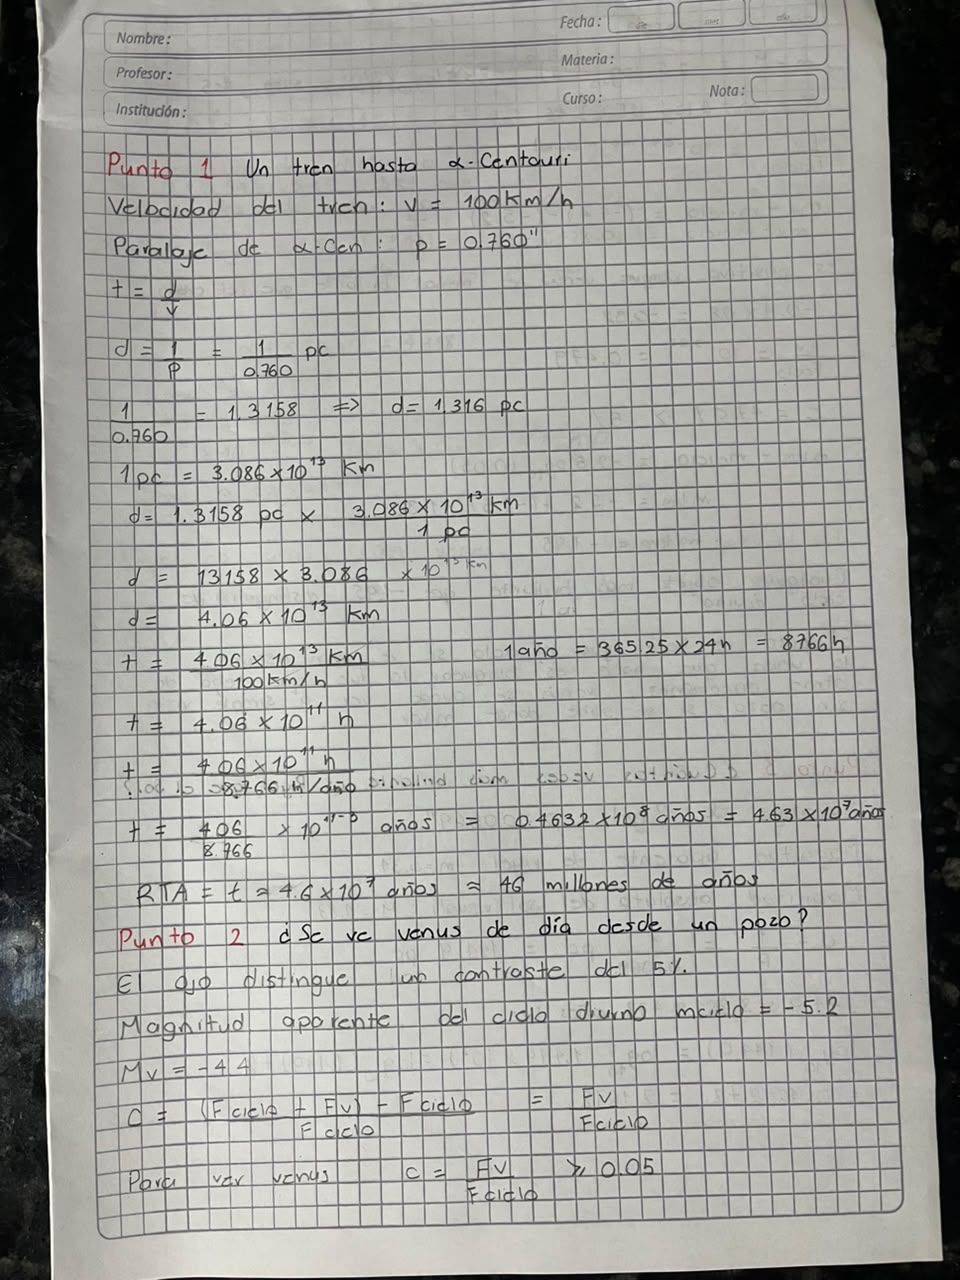
\includegraphics[height=0.82\textheight]{hoja1_puntos1_2.jpg}
\caption{Hoja 1: punto 1 completo y comienzo del punto 2.}
\end{figure}

\begin{figure}[H]
\centering
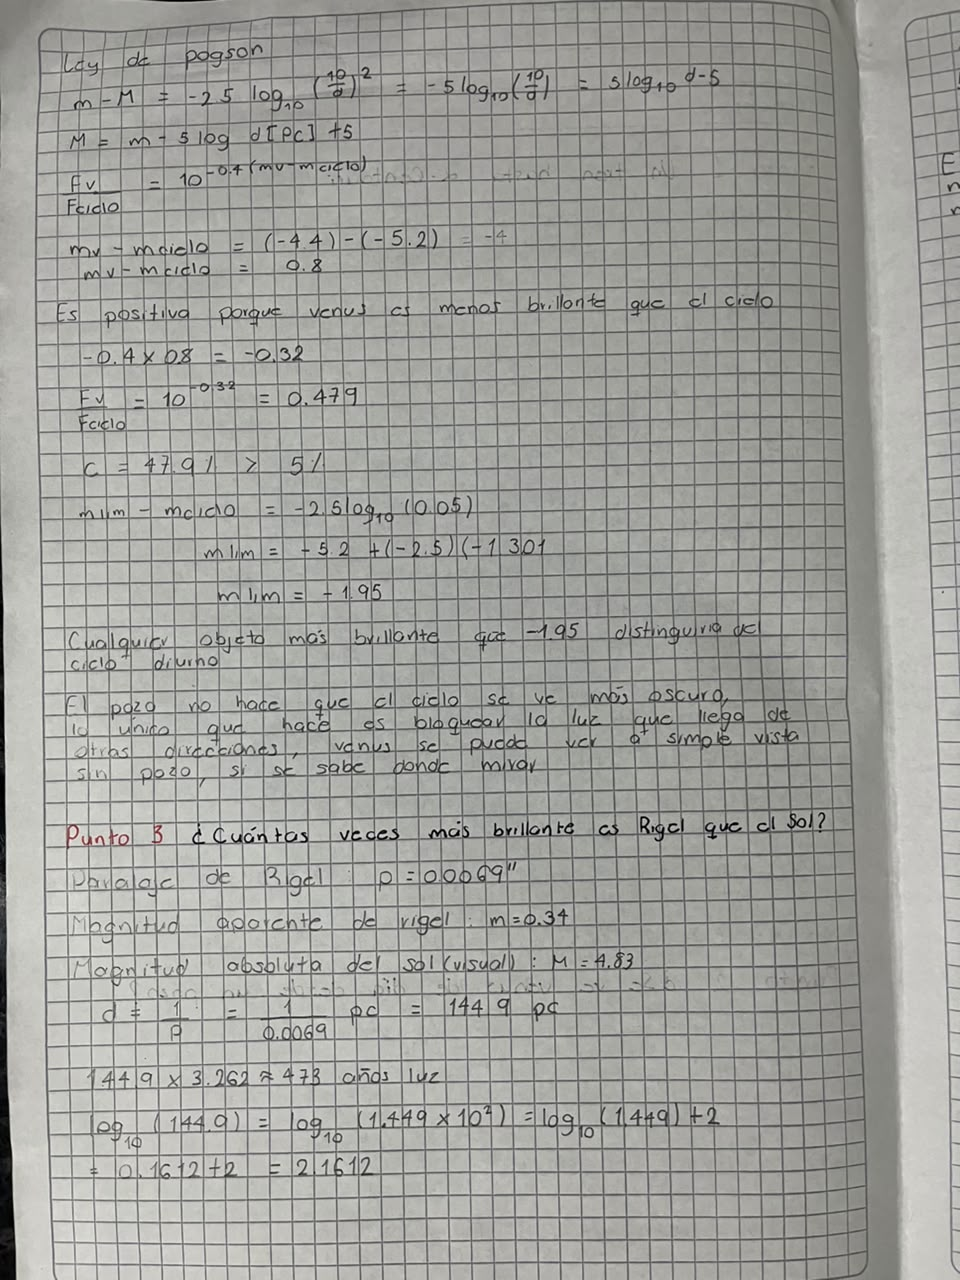
\includegraphics[height=0.82\textheight]{hoja2_puntos2_3.jpg}
\caption{Hoja 2: continuación del punto 2 y comienzo del punto 3.}
\end{figure}

\begin{figure}[H]
\centering
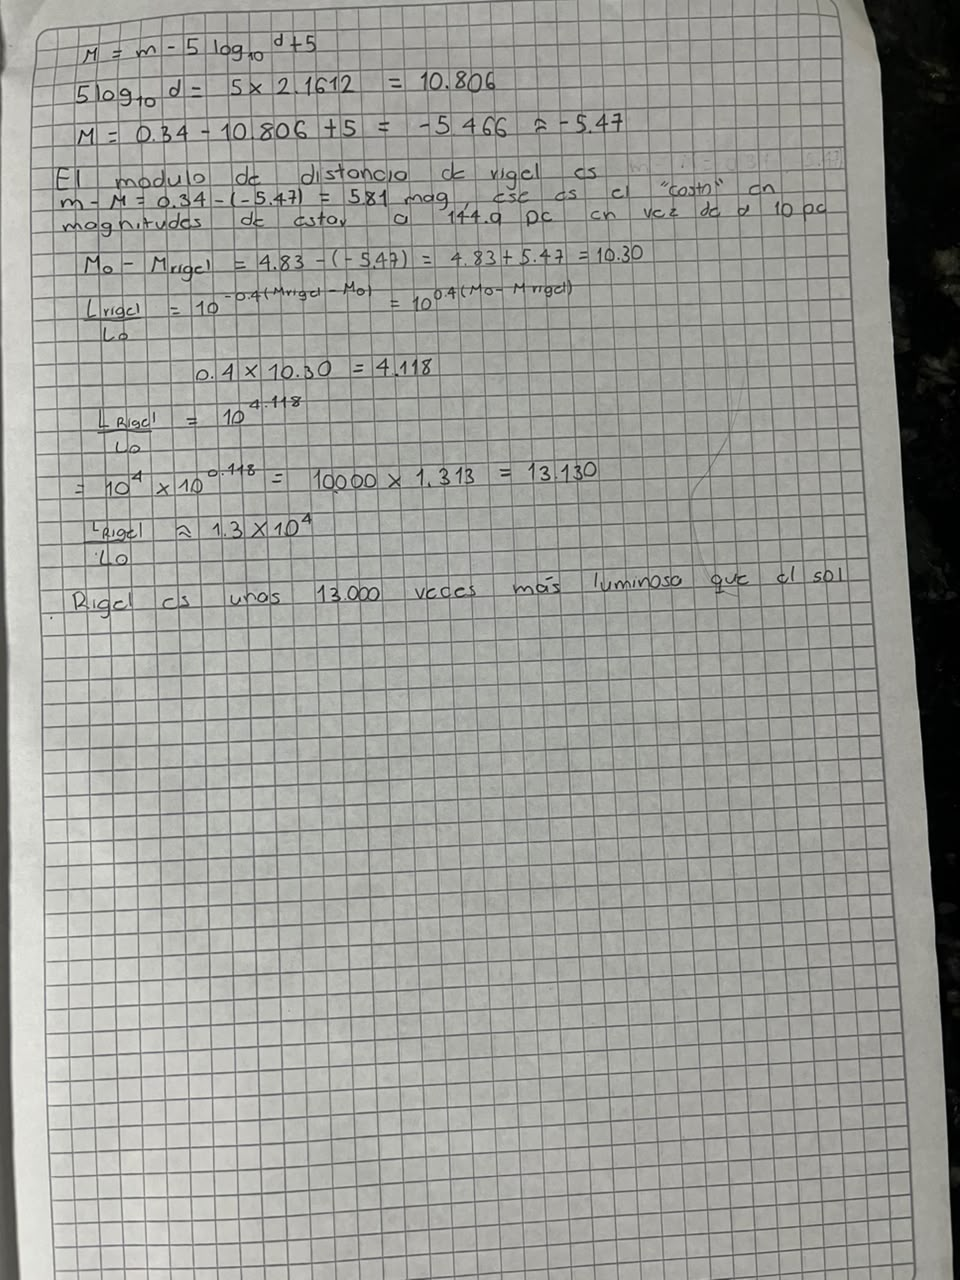
\includegraphics[height=0.82\textheight]{hoja3_punto3.jpg}
\caption{Hoja 3: final del punto 3.}
\end{figure}

\subsection{Punto 1: un tren a \texorpdfstring{$\alpha$}{alfa}~Centauri}
\begin{revision}
Procedimiento y resultado correctos: $d = 1/0.760 = \SI{1.316}{pc} = \SI{4.06e13}{km}$,
$t = \SI{4.06e11}{h} = \num{4.63e7}$ años $\approx$ \textbf{46 millones de años}.

Corrección menor de escritura: en la línea ``$d = 13158 \times 3.086 \times 10^{13}$'' falta el punto
decimal; debe decir $d = 1.3158 \times 3.086 \times 10^{13}$~km. El resultado de la línea siguiente
($\SI{4.06e13}{km}$) está bien.
\end{revision}

\subsection{Punto 2: ¿Venus de día desde el fondo de un pozo?}
\begin{revision}
Cálculo correcto: $m_V - m_\text{cielo} = -4.4 - (-5.2) = 0.8$;
$F_V/F_\text{cielo} = 10^{-0.32} = 0.479$, es decir 47.9\,\% $> 5$\,\%; y
$m_\text{lím} = -5.2 + 2.5\log_{10}(20) = -1.95$. También es correcto que el pozo no oscurece el cielo.
\end{revision}

\begin{complemento}
\textbf{1. Origen del dato $m_V = -4.4$.} No está en el enunciado. Es la magnitud de Venus en su
máximo brillo, que llega a $-4.4$ a $-4.6$ según el Observatorio Astronómico Nacional de Japón (NAOJ).

\textbf{2. El argumento geométrico.} Desde el fondo de un pozo profundo solo se ve una zona pequeña
del cielo alrededor del cenit: un pozo de \SI{1}{m} de diámetro y \SI{20}{m} de profundidad muestra
un círculo de $\arctan(0.5/20) \approx 1.4^\circ$ de radio. Venus nunca se aleja más de unos
$27$--$28^\circ$ del ecuador celeste (la eclíptica está inclinada $23.4^\circ$ y la órbita de Venus
otros $3.4^\circ$). En Albania, a unos $41^\circ$ de latitud norte, Venus pasa como mínimo a unos
$41^\circ - 28^\circ = 13^\circ$ del cenit, así que nunca entra en el trozo de cielo visible desde el
pozo.

\textbf{3. Respuesta explícita a la pregunta.} \emph{La afirmación no merece crédito.} Por brillo,
Venus sí se puede ver de día (su contraste es casi diez veces el mínimo que distingue el ojo), y se ve
sin necesidad de un pozo. Pero el pozo no ayuda, porque no oscurece el cielo. Y desde el fondo de un
pozo profundo en Albania, Venus nunca pasa por la pequeña zona de cielo visible.
\end{complemento}

\subsection{Punto 3: ¿cuántas veces más brillante es Rigel que el Sol?}
\begin{revision}
Todo correcto: $d = 1/0.0069 = \SI{144.9}{pc}$ ($\approx 473$ años luz),
$\log_{10}(144.9) = 2.1612$, $M = 0.34 - 10.806 + 5 = -5.47$, módulo de distancia $5.81$~mag, y
$L_\text{Rigel}/L_\odot = 10^{4.118} \approx \num{13130}$.
\end{revision}

\begin{complemento}
\textbf{Banda de la luminosidad.} Como se usó $M_\odot = 4.83$, que es la magnitud absoluta del Sol en
la banda visual (V), el resultado compara la \emph{luz visible}: ``Rigel emite unas \num{13000} veces
más luz visible que el Sol''. Rigel es una supergigante azul (B8\,Ia) que emite mucho en el
ultravioleta, así que su luminosidad total es aún mayor.

\textbf{Comparación con datos actuales (opcional).} SIMBAD da hoy para Rigel una paralaje de
$3.78 \pm 0.34$~mas y $V = 0.13$. Con esos valores, $d \approx \SI{265}{pc}$ y
$L/L_\odot \approx \num{5.3e4}$ en la banda visual.
\end{complemento}

% =====================================================================
\section{Punto 4: la Gran Nube de Magallanes}
\begin{complemento}[title={Complemento: punto 4 completo (no estaba en las hojas)}]
Todo este punto es nuevo. Se usaron imágenes de NASA SkyView, porque los servidores del CDS
(Estrasburgo) no respondieron, y la distancia de la LMC, \SI{50}{kpc}.
\end{complemento}

\subsection{Visualización en cuatro bandas}
\begin{figure}[H]
\centering
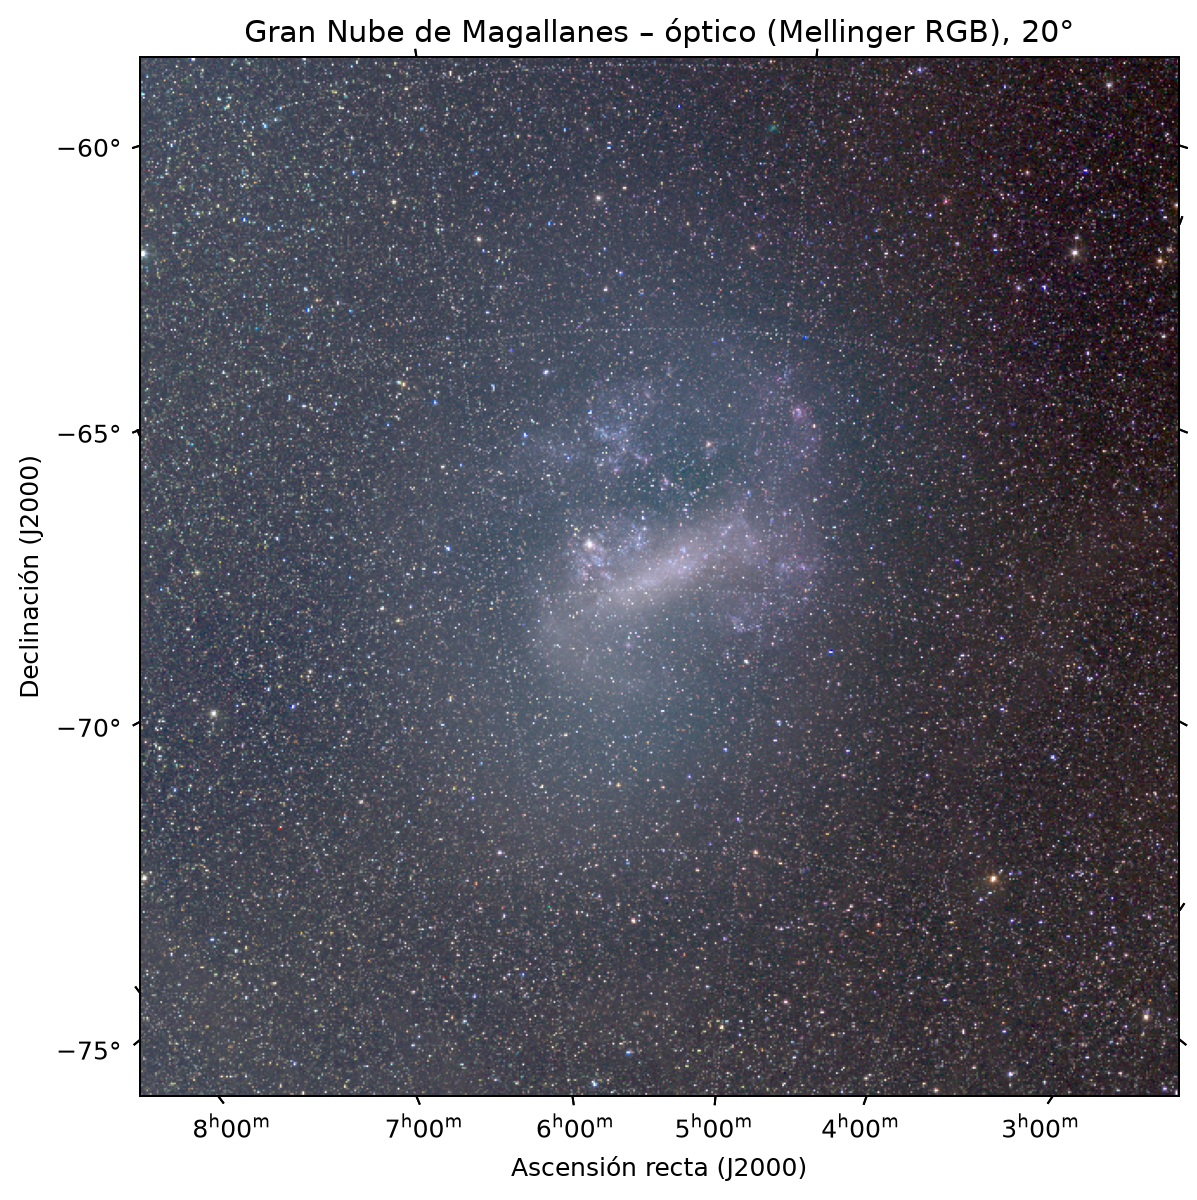
\includegraphics[width=0.40\textwidth]{punto4/LMC_optico_Mellinger_color_20deg.png}
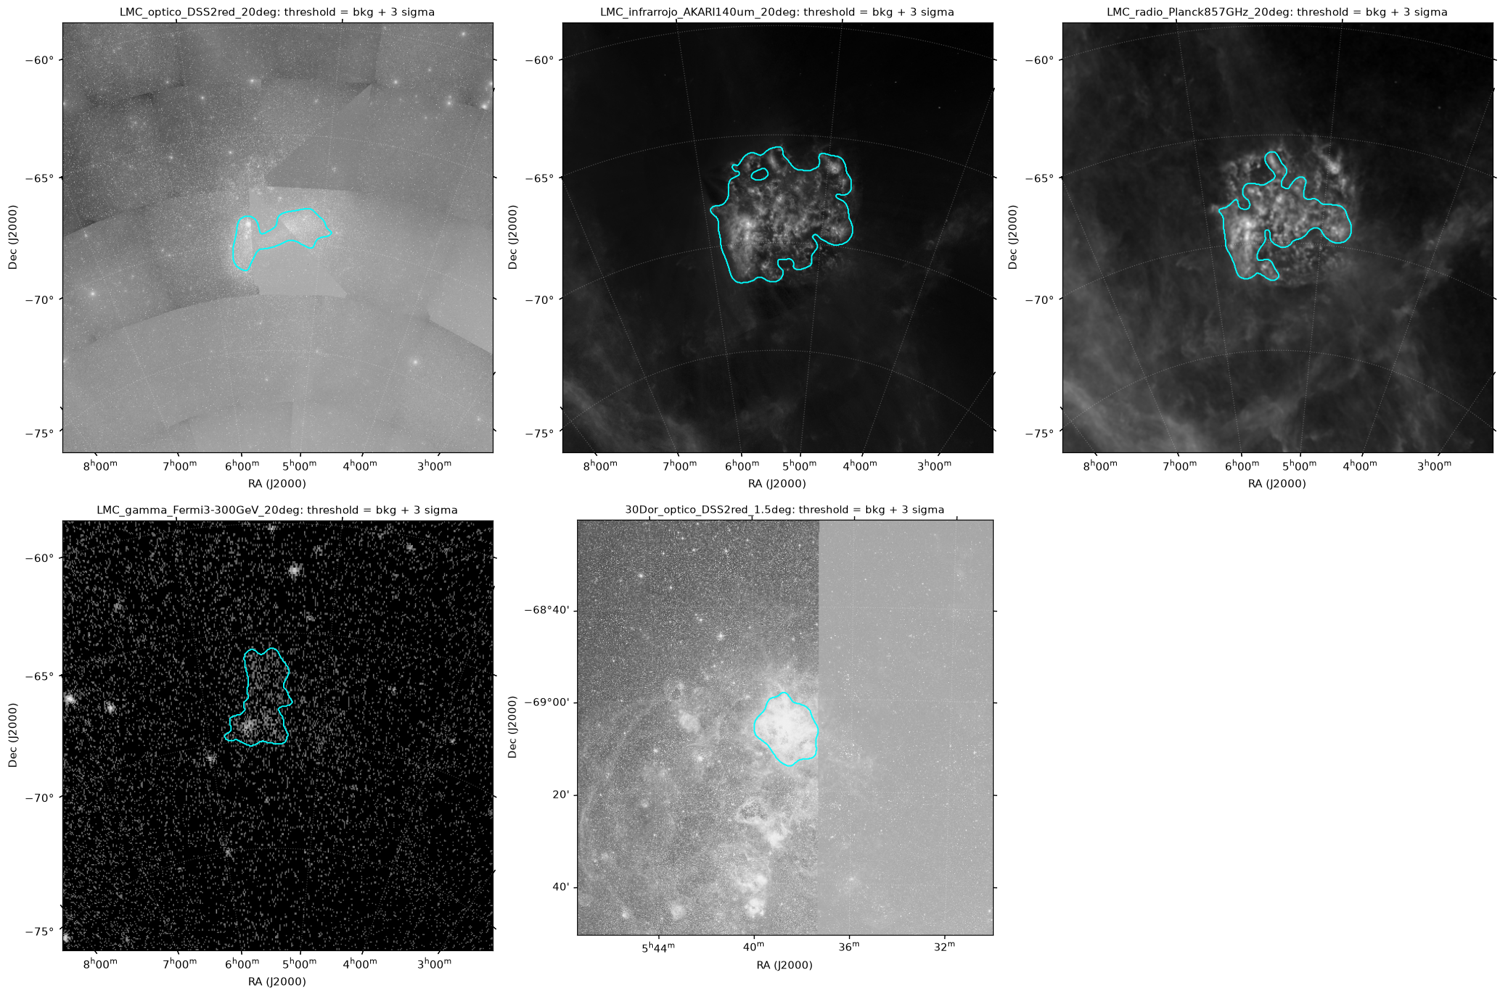
\includegraphics[width=0.58\textwidth]{punto4/panel_medidas_umbral3.png}
\caption{Izquierda: la LMC en óptico (Mellinger), con la barra central y el disco difuso. Derecha:
contorno de medida en óptico, infrarrojo (AKARI \SI{140}{\micro m}), submilimétrico (Planck
\SI{857}{GHz}), radio (Planck \SI{30}{GHz}), rayos gamma (Fermi) y la Nebulosa de la Tarántula
(30~Doradus).}
\end{figure}

\subsection{(a) Diámetro angular en cada imagen}
Se midió de dos formas. La \textbf{automática} marca los píxeles por encima de fondo $+\,3\sigma$ y mide
la región central. La \textbf{regla} sigue el brillo a lo largo de cada eje y pone el borde donde cae
al cielo vecino más un 10\,\% del contraste, como al medir con la herramienta de distancia de Aladin.

\begin{table}[H]
\centering
\caption{Diámetro angular de la LMC en cada banda (eje mayor $\times$ eje menor).}
\small
\begin{tabular}{lccc}
\toprule
Banda & Automática ($3\sigma$) & Con regla & Referencia \\
\midrule
Óptico & $4.87^\circ \times 2.42^\circ$ & $11.33^\circ \times 8.27^\circ$ & RC3: $10.76^\circ \times 9.16^\circ$ \\
Infrarrojo (AKARI) & $6.98^\circ \times 5.51^\circ$ & $6.43^\circ \times 4.80^\circ$ & -- \\
Submm (Planck 857 GHz) & $6.14^\circ \times 4.54^\circ$ & $6.53^\circ$ (eje mayor) & -- \\
Radio (Planck 30 GHz) & $5.66^\circ \times 5.39^\circ$ & $7.10^\circ \times 5.60^\circ$ & -- \\
Gamma (Fermi) & $5.10^\circ \times 3.08^\circ$\,$^*$ & no medible$^\dagger$ & -- \\
30 Doradus & $15.5' \times 12.4'$ & $37.5' \times 30.0'$ & SIMBAD: $40' \times 25'$ \\
\bottomrule
\multicolumn{4}{l}{\footnotesize $^*$ Mapa suavizado con $\sigma = 0.5^\circ$ (cota superior). $^\dagger$ En el mapa crudo solo hay fotones sueltos.}
\end{tabular}
\end{table}

\textbf{¿Qué resultados se obtienen?} El tamaño cambia con la longitud de onda porque cada banda ve un
componente distinto:
\begin{itemize}
  \item el \textbf{óptico}, la luz de las estrellas: la barra brillante y un disco externo débil;
  \item el \textbf{infrarrojo}, el polvo frío calentado por estrellas jóvenes, repartido por todo el disco;
  \item el \textbf{submilimétrico}, polvo aún más frío;
  \item la \textbf{radio}, el gas ionizado de las regiones de formación estelar;
  \item los \textbf{rayos gamma}, los rayos cósmicos que chocan con el gas. Hay pocos fotones, así que la
  emisión solo aparece al suavizar el mapa.
\end{itemize}
El resultado también depende del criterio de borde. El método automático deja afuera el halo débil, y
con la regla el óptico coincide con el catálogo RC3.

\textbf{Tamaño físico} ($D = d\,\theta$, con $\theta$ en radianes): con la regla en óptico,
$D = \SI{50}{kpc} \times 11.33^\circ \times \pi/180 \approx \SI{9.9}{kpc}$; en infrarrojo (AKARI,
automática), $\approx \SI{5.2}{kpc}$. La nebulosa 30~Doradus ($37.5'$) mide $\approx \SI{0.55}{kpc}$.

\subsection{(b) Estrellas masivas de Bonanos et al.\ (2009)}
El catálogo (VizieR J/AJ/138/1003, tabla~3) tiene 1268 estrellas masivas. No trae una columna B$-$V:
se calcula como $\text{Bmag} - \text{Vmag}$. Quedan 1100 estrellas válidas; otras 35 tienen colores
físicamente imposibles y se graficaron aparte.

\begin{figure}[H]
\centering
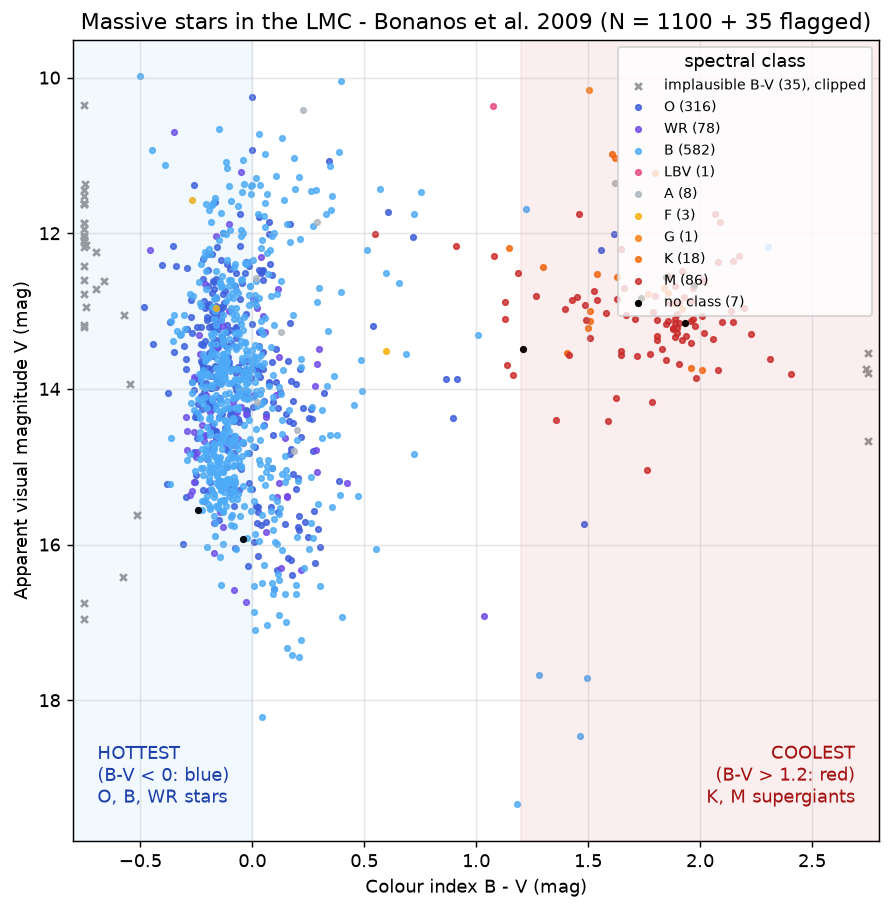
\includegraphics[width=0.49\textwidth]{punto4/Bonanos2009_LMC_V_vs_BV.png}
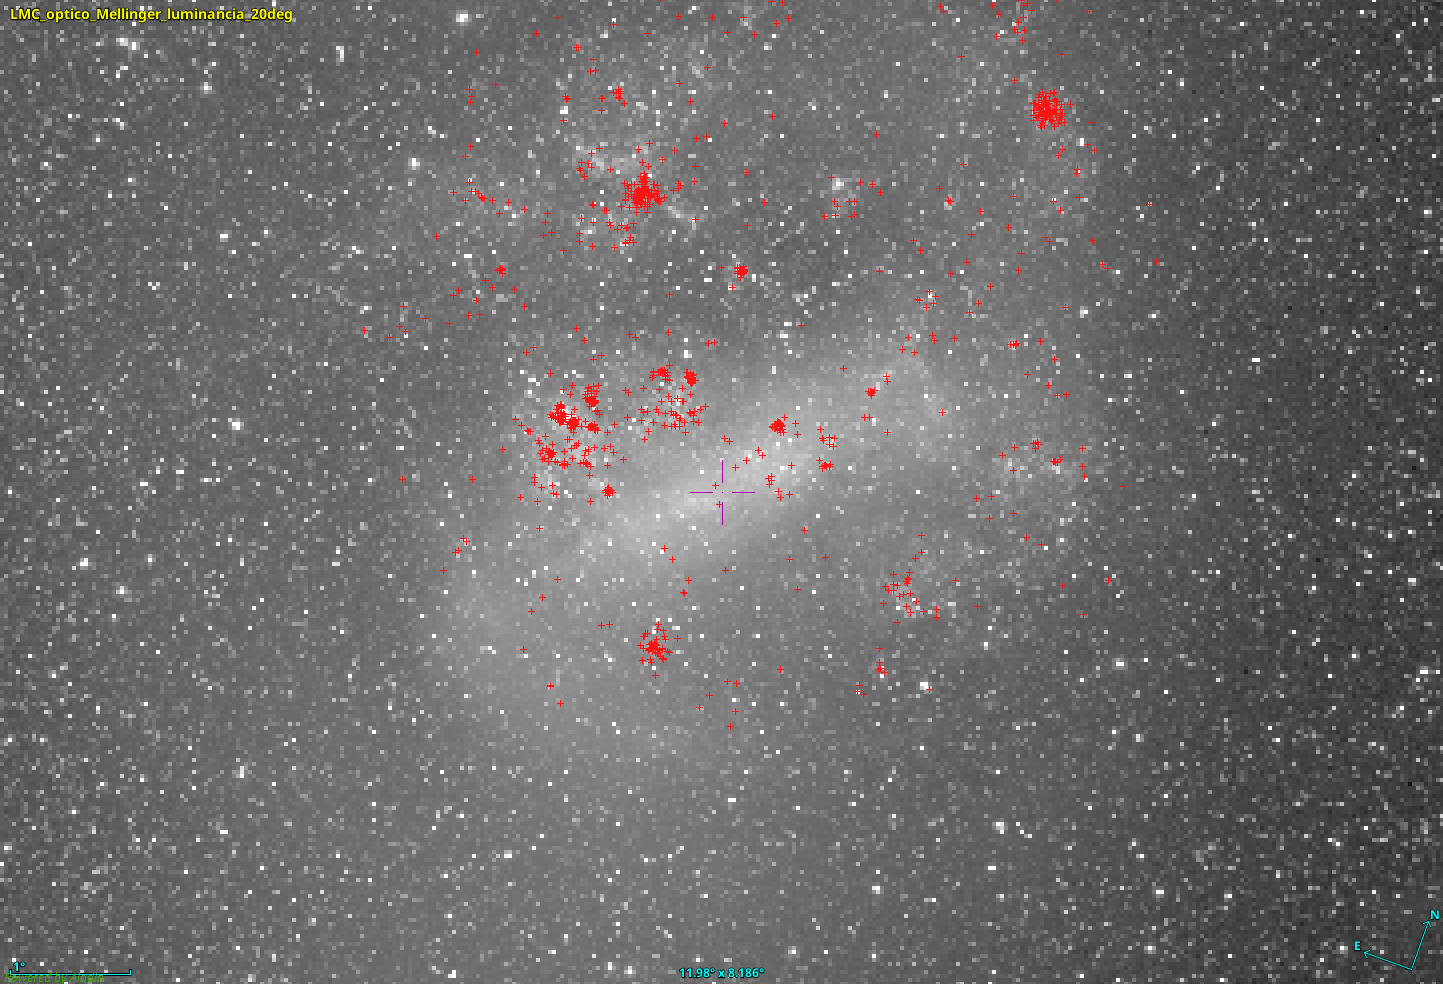
\includegraphics[width=0.49\textwidth]{capturas/aladin_Bonanos2009_sobre_LMC.png}
\caption{Izquierda: magnitud visual V (eje invertido) contra índice de color B$-$V. Derecha: las
estrellas localizadas sobre la imagen en Aladin; se concentran en la barra y en 30~Doradus.}
\end{figure}

\subsection{(c) Estrellas frías y calientes en el diagrama}
\textbf{a) Las de superficie más fría están a la derecha} ($B-V$ entre $+1.2$ y $+2.4$): son
supergigantes rojas K y M (B$-$V medio $+1.66$ y $+1.76$), con superficies de unos
\SIrange{3500}{4500}{K}.

\textbf{b) Las más calientes están a la izquierda} ($B-V \approx 0$ o negativo): estrellas O, B y
Wolf-Rayet (B$-$V medio $-0.05$, $-0.03$ y $-0.06$), con superficies de \SI{20000}{K} a más de
\SI{40000}{K}.

\textbf{¿Por qué?} B mide la luz azul (\SI{\sim 440}{nm}) y V la visual (\SI{\sim 550}{nm}). Por la ley de
Wien, $\lambda_\text{máx} = b/T$: una estrella de \SI{30000}{K} emite sobre todo en \SI{97}{nm} y
brilla más en B que en V, así que $B-V < 0$. Una de \SI{3500}{K} emite sobre todo en \SI{828}{nm} y
brilla más en V, así que $B-V$ es grande. El polvo enrojece a las estrellas: las O deberían estar en
$B-V \approx -0.3$ y su promedio observado es $-0.05$.

% =====================================================================
\section{Punto 5: la edad de la Caja de Joyas (NGC 4755)}

\begin{figure}[H]
\centering
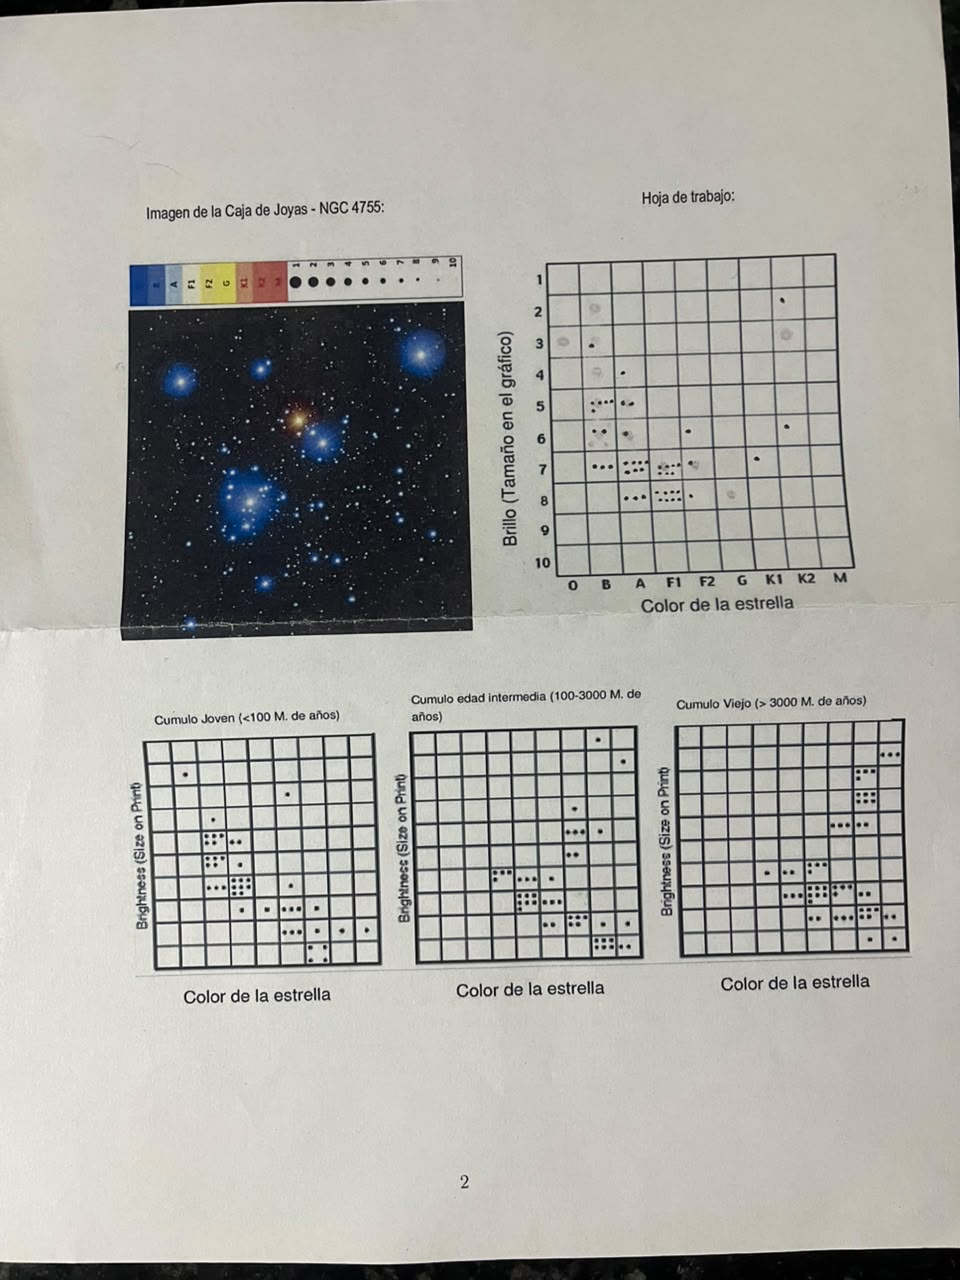
\includegraphics[height=0.72\textheight]{hoja4_punto5.jpg}
\caption{Hoja 4 (página 2 del taller): hoja de trabajo llenada a mano.}
\end{figure}

\begin{revision}
La hoja de trabajo está llena y los puntos están en casillas coherentes:
\begin{itemize}
  \item estrellas B brillantes arriba a la izquierda (brillos 3 a 7);
  \item la diagonal de estrellas A y F1 en brillos 7 y 8;
  \item una estrella roja muy brillante (K2, brillo 2), la supergigante roja DU~Cru.
\end{itemize}
\end{revision}

\begin{complemento}[title={Complemento: (1) centro, límite y cuadrado en la foto}]
La foto del cúmulo no tenía marcas. La figura~\ref{fig:marcas} muestra:
\begin{itemize}
  \item el \textbf{centro} (X roja), entre la estrella naranja (DU~Cru), la azul que está justo debajo
  (BU~Cru) y el grupo azul de abajo a la izquierda ($\kappa$~Cru);
  \item el \textbf{límite} (círculo amarillo), donde la cantidad de estrellas baja al nivel del fondo;
  \item el \textbf{cuadrado} (verde) donde se estimaron el brillo y el color de las 46 estrellas
  numeradas.
\end{itemize}
\end{complemento}

\begin{figure}[H]
\centering
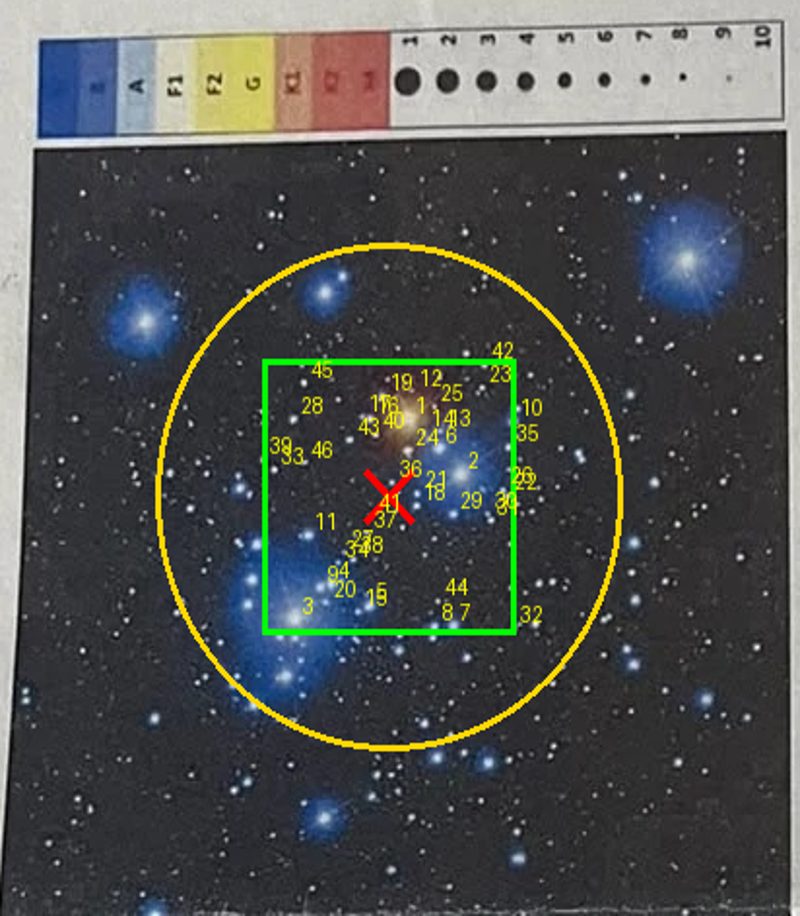
\includegraphics[width=0.48\textwidth]{punto5/pagina2_cumulo_ampliado.png}
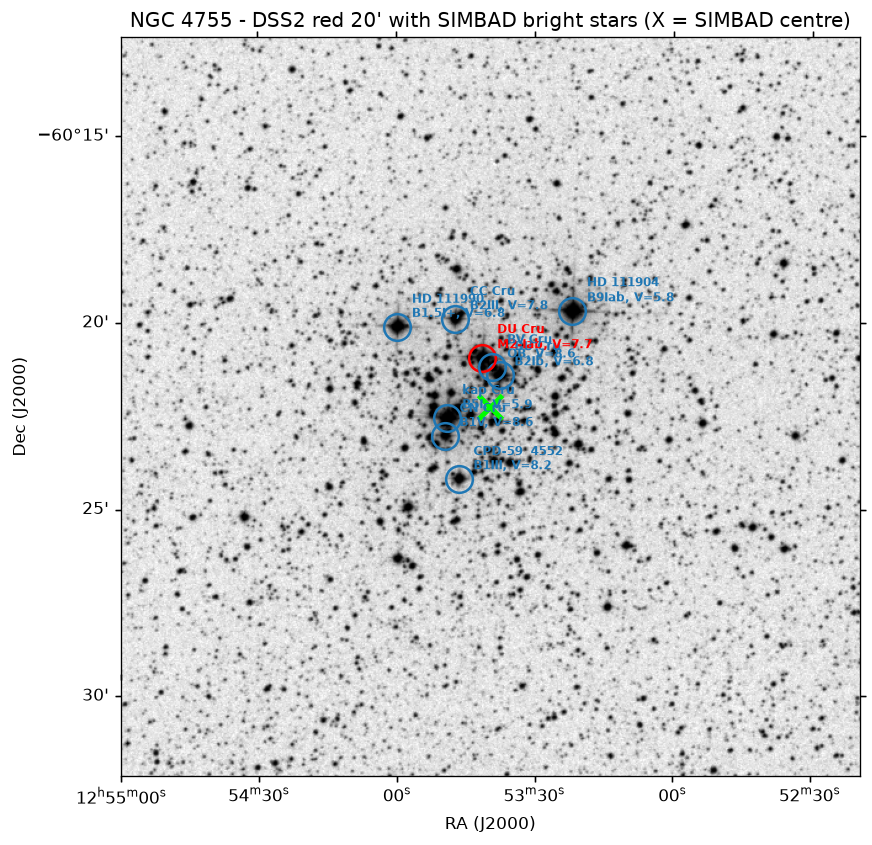
\includegraphics[width=0.48\textwidth]{punto5/NGC4755_DSS2red_estrellas_identificadas.png}
\caption{Izquierda: la foto del taller con el centro, el límite y el cuadrado. Derecha: el mismo
cúmulo con sus estrellas brillantes identificadas en SIMBAD.}
\label{fig:marcas}
\end{figure}

\begin{complemento}[title={Complemento: (2) estimación de la edad}]
Al comparar la hoja de trabajo con los tres diagramas de referencia:
\begin{itemize}
  \item un cúmulo \textbf{joven} ($< 100$ millones de años) tiene estrellas azules muy brillantes arriba
  a la izquierda;
  \item uno de \textbf{edad intermedia} (100 a 3000 millones) ya no las tiene y muestra gigantes rojas;
  \item uno \textbf{viejo} ($> 3000$ millones) solo conserva la parte baja de la secuencia y muchas
  gigantes rojas.
\end{itemize}
La hoja de trabajo tiene estrellas B muy brillantes arriba a la izquierda y una sola supergigante roja,
y no muestra el grupo de gigantes rojas de los cúmulos más viejos. Por lo tanto, \textbf{la Caja de
Joyas es un cúmulo joven, de menos de 100 millones de años}. La literatura le da entre 10 y 16 millones
de años (Sanner et al.\ 2001; Bonatto et al.\ 2006; Piskunov et al.\ 2004).

El diagrama real de Gaia (figura~\ref{fig:gaia}) lo confirma. Las estrellas B más brillantes ya
empiezan a salir de la secuencia principal, y eso solo ocurre tan arriba en un cúmulo muy joven.
\end{complemento}

\begin{figure}[H]
\centering
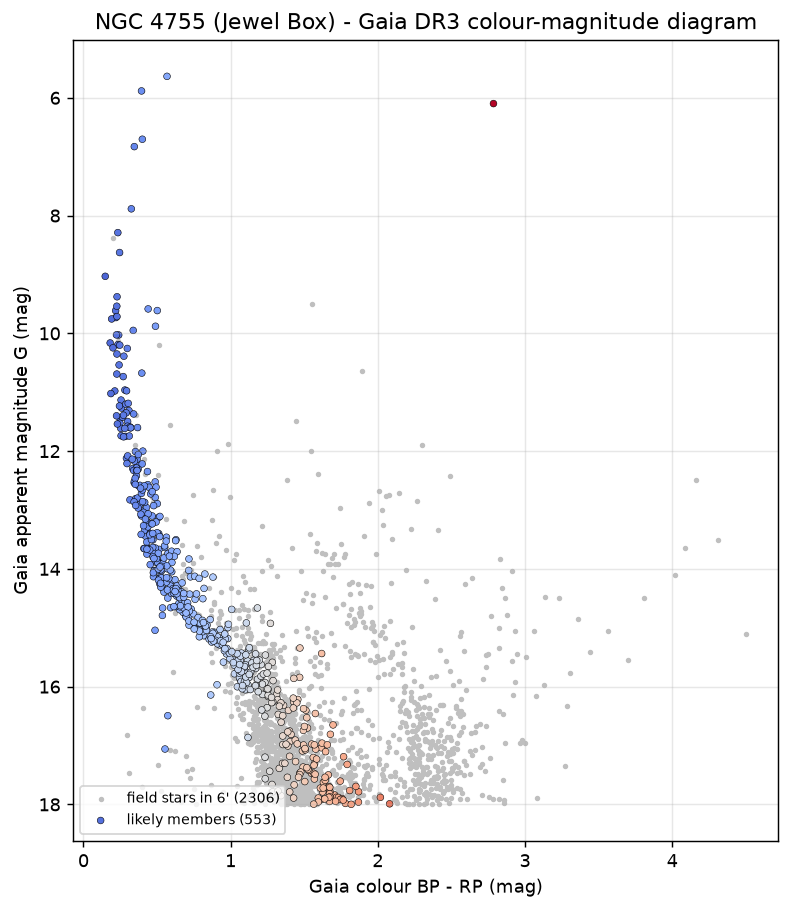
\includegraphics[width=0.58\textwidth]{punto5/NGC4755_GaiaDR3_CMD.png}
\caption{Diagrama color-magnitud de NGC~4755 con 553 miembros de Gaia DR3. El recuadro verde marca el
punto de giro, en lo más alto del diagrama.}
\label{fig:gaia}
\end{figure}

% =====================================================================
\section{Pendiente para completar a mano}
\begin{itemize}
  \item El \textbf{encabezado} de la primera hoja: nombre, profesor, institución, fecha, materia y curso.
  \item Si la entrega es en papel: dibujar la X, el círculo y el cuadrado sobre la foto del cúmulo,
  siguiendo la figura~\ref{fig:marcas}, y copiar la conclusión del punto 5\,(2).
\end{itemize}

\end{document}
